\def\chapname{A Space-Frequency Localization Algorithm}
\chapter[\chapname]{
\chapname \chapsubhead{The results of this chapter are published in \cite{ABG2012modeling}.}}
\label{chap:localization}

\begin{abstract}
Based on the dipole approximation shown in the previous chapter,
we obtain here a non-iterative location search algorithm using 
multi-frequency measurements. We
present numerical experiments to illustrate the performance and
the stability of the algorithm. In the case of disk- and 
ellipse-shaped
targets, we provide a method to reconstruct separately the
conductivity, the permittivity, and the size of the targets from
multi-frequency measurements.
\end{abstract}

\section{Introduction}

\label{sec:intro-localization}

For the inverse problem, little is known in the
complex admittivity case \cite{berettafrancini2011stability}. Here, we take advantage
of the smallness of the targets to use the framework of small
volume asymptotic expansions (see section~\ref{sub:dipolar-expansion}) for target location and
characterization \cite{ammari2004reconstruction,
ammari2007polarization}. However, since the electric current is
generated by only one emitter at the tail of the fish (the
electric organ) and measured by many receptors on the skin,
standard non-iterative algorithms such as MUSIC (standing for
MUltiple Signal Classification) cannot be applied for location
search. In standard MUSIC, the data (called multistatic response
matrix) form a matrix and its singular value decomposition leads
to an efficient imaging function by projecting the Green function
of the medium onto the significant image space
\cite{AGKPS2011cracks,AIL2005music,AKKLV2008music, bruhl2003direct, chambersberryman2006target, cheney2001linearsampling,
kirsch1999characterization}. Here, roughly speaking, one has only a column of the
response matrix. However, using the fact that the electric current
produced by the electric organ is time-harmonic with a known
fundamental frequency, we extend MUSIC approach to multi-frequency
measurements by constructing an efficient and robust
multi-frequency MUSIC imaging function. We perform numerical
simulations in order to validate both the direct model and the
multi-frequency MUSIC algorithm. We also illustrate the robustness
with respect to measurement noise and the sensitivity with respect
to the number of frequencies, the number of sensors, and the
distance to the target of the location search algorithm. Finally,
in the case of disk- and ellipse-shaped targets, we provide a
method to reconstruct separately the conductivity, the
permittivity, and the size of the targets from multi-frequency
measurements. We mention that this is possible only because of
multi-frequency measurements which yield polarization tensors with
complex admittivty. It is well-known that polarization tensors
for vanishing capacitance (\ie real-valued admittivity) cannot separate the size from material
properties of the target \cite{ammari2007polarization}. We also
mention that the use of different values for the frequencies is
more crucial for the material and size reconstruction procedure
than for the location step. In fact, in the presence of
measurement noise, location with $N_f$ realizations with one
frequency is comparable to the one with $N_f$ different frequency
values.

\section{Detection algorithm for multi-frequency measurements}

\label{sec:detection_algo}

Scholz described in \cite{scholz2002towards} a way to recover the
location of a target from multi-frequency measurements. The paper
focuses on an application in electrical impedance tomography (EIT)
for breast cancer detection; the algorithm was called
``Space-Frequency MUSIC''. Indeed, it is based on the so-called
MUSIC algorithm, which is a standard tool in signal theory for the
identification of several signals with an additive noise
\cite{schmidt1986multiple, devaney2004super}. It has then been
applied to identify small conductivity inhomogeneities in
\cite{ammari2007identification, AKKLV2008music, bruhl2003direct}. In this section,
we apply a similar approach for our model.

In this section, we develop an algorithm to recover (from a single
measurement) the location of a small object located far away from
the fish. This algorithm is based on multi-frequency measurements defined in
subsection~\ref{sub:response-matrix}, and the algorithm will be explained in
detail in subsection~\ref{sub:algorithm}.

\subsection{Response matrix}

\label{sub:response-matrix}

The electroreceptors of the fish measure the electric current at
the surface of the skin \cite{moller1995electric}. Hence, from a single
measurement, we can construct the Space-Frequency Response (SFR)
matrix $\mathbf{V}$, whose terms are given by
\[
V_{rf}=\left(\left.\frac{\partial
u_{f}}{\partial\nu}\right|_{+}-\left.\frac{\partial
U}{\partial\nu}\right|_{+}\right)(x_{r}),\,\,\textrm{ for } 1\leq
f\leq N_f\textrm{ and }1\leq r\leq N_r,
\]
 where $\left(x_{r}\right)_{1\leq r\leq N_r}$ are points on the boundary
$\Gamma$ and $U$ is the static background solution, \emph{i.e.},
the electric potential without any target which does not depend on
$f$. It is the solution of (\ref{eq:complex_neumann_problem}) with
a constant conductivity equal to $1$ outside the body $\Omega$.

Recalling from section~\ref{sec:perturbation-target}, after a calculation of $\left.\frac{\partial
u_{f}}{\partial\nu}\right|_{+}-\left.\frac{\partial
U}{\partial\nu}\right|_{+}$ on $\Gamma$, we will apply the
post-processing operator given in Lemma \ref{lemgreen}. The
modified matrix will still be denoted $A$.

Thus, the location of the target $D$ is going to be
recovered from the knowledge of the following data
\begin{equation} \label{defdata}
\begin{alignedat}{1}V_{rf} & =\left(\frac{1}{2}I-\mathcal{K}_{\Gamma}^{*}-\xi\frac{
\partial\mathcal{D}_{\Gamma}}{\partial\nu}\right)\left(\left.\frac{\partial u_{f}}{\partial\nu}\right|_{+}-\left.
\frac{\partial U}{\partial\nu}\right|_{+}\right)(x_{r}), \quad 1\leq r\leq N_r, 1 \leq f\leq N_f, \\
\end{alignedat}
\end{equation}
which is approximately equal to
\begin{equation}
\begin{alignedat}{1}V_{rf}
 & \simeq \delta^{2}\nabla U(z)^T \mathbf{M}(\lambda_{f},B) \nabla_{z}\left(\left.\frac{\partial G}{\partial\nu_{x}}\right|_{+}
 \right)(x_{r},z),
\end{alignedat}
\label{eq:SFR-final}
\end{equation}
when the characteristic size of the target $\delta$  is small. It
is worth mentioning that the  polarization tensor $\mathbf{M}(\lambda_{f},B)$ is
symmetric (but not Hermitian) \cite{ammari2007polarization}.


\subsection{A location search algorithm}

\label{sub:algorithm}

As we can see in formula (\ref{eq:SFR-final}), the rows of the SFR
matrix are - to leading-order - linear combinations of the
derivatives of $\partial G/\partial\nu_{x}$. Moreover, one has to
distinguish whether the target is a disk or not. Indeed, in
dimension $2$ and in the case of an ellipse whose semi-axes are on
the $x_{i}$-axis and of length $a$ and $b$, the polarization
tensor $\mathbf{M}(\lambda,B)$, for $k\in \mathbb{C}$,  takes the form
\cite{milton2002theory}
\[
\mathbf{M}(\lambda,B)=(k-1)\vert B\vert\left(\begin{array}{cc}
\frac{a+b}{a+kb} & 0\\
0 & \frac{a+b}{b+ka}
\end{array}\right).
\]
%Note that in \cite{bruhl2003direct}, the calculation was made for
%$k\in\mathbb{R}$, but it remains correct for $k\in\mathbb{C}$.
Hence, the polarization tensor is proportional to the identity
matrix if and only if $a=b$, \emph{i.e.}, $B$ is a disk; this
result remains true in dimension $3$
\cite{ammari2007polarization}. This changes dramatically the range
of $A$: if $B$ is a disk, the response matrix
has rank $1$ and if it is an ellipse, it has rank $2$.\\
For the sake of simplicity, let us suppose that $B$ is the unit disk.
The identification process will be based on the following fact

\begin{lemma}\label{lemma:one-to-one}The following map
\[\begin{array}{ll}
\Lambda: &\mathbb{R}^{2}\setminus\overline{\Omega} \rightarrow  L^{2}(\Gamma)\\
\nm &z \mapsto  \nabla U(z)^T \nabla_{z}\frac{\partial
G}{\partial\nu_{x}}(\cdot,z),
\end{array}
\]
is one-to-one.\end{lemma}

\proof

Suppose that $z$ and $z'$ are points on
$\mathbb{R}^{2}\setminus\overline{\Omega}$ such that
$\Lambda(z)=\Lambda(z'):=\varphi$. Let us define the two following
functions
\[
\begin{array}{ll}v_{z}: &\mathbb{R}^{2}\setminus\overline{\Omega}\cup\{z\} \rightarrow \mathbb{R}\\
& x \mapsto  \nabla U(z)^T \nabla_{z}G(x,z),
\\
\nm \nm \nm
v_{z'}: & \mathbb{R}^{2}\setminus\overline{\Omega}\cup\{z'\} \rightarrow  \mathbb{R}\\
& x \mapsto  \nabla U(z')^T \nabla_{z'}G(x,z').
\end{array}
\]
Thus, these two functions both solve the following boundary value
problem
\[
\left\{ \begin{alignedat}{2}\Delta v & =0, & \,\, x\in\mathbb{R}^{2}\setminus\overline{\Omega}\cup\{z\}\cup\{z'\},\\
\frac{\partial v}{\partial\nu} & =\varphi, & \,\, x\in\Gamma,\\
v & \rightarrow0 & \,\,\left|x\right|\rightarrow\infty,\text{ uniformly in }\hat{x}.
\end{alignedat}
\right.
\]
Hence, by the uniqueness of the solution for this problem, we have
\[
\nabla U(z)\cdot\nabla_{z}G(x,z)=\nabla
U(z')\cdot\nabla_{z'}G(x,z'),\mbox{ for all
}x\in\mathbb{R}^{2}\setminus\overline{\Omega}\cup\{z\}\cup\{z'\}.
\]
Relying on the singularity of $G(\cdot,z)$ at the point $z$, this
is only possible if $z=z'$.

\cqfd

However, we do not have access to the complete function (because
there is only a finite number of electroreceptors on the body),
and the formula for $\Lambda$ is only an approximation, based
on~(\ref{eq:SFR-final}). The location of the target will then be
approximated as follows. In the following we suppose for the sake
of simplicity that $x_1,\ldots, x_L$ are equi-distributed on
$\Gamma$.

\begin{proposition}[Space-Frequency MUSIC]

\label{proposition:SF-MUSIC} Define the vector
\begin{equation}
\tilde{g}(z):=\left(\nabla U(z)\cdot\nabla_{z}\left(\frac{\partial
G}{\partial\nu_{x}}\right)(x_{1},z),\ldots,\nabla
U(z)\cdot\nabla_{z}\left(\frac{\partial
G}{\partial\nu_{x}}\right)(x_{N_r},z)\right)^{T},\label{eq:illumination-vector-disk}
\end{equation}
and its normalized version $g=\tilde{g}/\vert\tilde{g}\vert$.
Then, in the limit $N_r\rightarrow+\infty$ and $\delta
\rightarrow0$, the following imaging functional will have a large
peak at $z$:
\begin{equation}
\mathcal{I}(z_{s}):=\frac{1}{\left|(I-P)g(z_{s})\right|},\label{eq:imaging_functional}
\end{equation}
 where $P$ is the orthogonal projection onto the first
singular vector of the SFR matrix $A$.

\end{proposition}

\proof

First of all, let us rewrite (just for this proof) the projection
$P_{\delta}^{N_r}$ and the illumination vector $g^{N_r}$, in order to
take into account the dependence with respect to $N_r$. When $N_r$
goes to infinity, quadrature formulas show us that
\[
\vert(I-P_{\delta}^{N_r})g^{N_r}(z_{s})\vert_{\mathbb{R}^{N_r}}\rightarrow\left|(I-P_{\delta})
\frac{\Lambda(z_{s})}{\vert\Lambda(z_{s})\vert_{L^{2}(\Gamma)}}\right|_{L^{2}(\Gamma)}.
\]
Here, $P_{\delta}$ is the projection onto the first singular
vector of the operator $\mathbb{A}_{\delta}$, acting on the space
of functions that have the form  (\ref{eq:formule-h})
\[\begin{array}{rll}
\mathbb{A}_{\delta}:  L^2[0, {2\pi}/{\omega_0}] &\rightarrow & L^2[0, {2\pi}/{\omega_0}] \times L^2(\Gamma) \\
\nm
\ds h = \sum_{f=1}^{N_f} h_r e^{i f \omega_0 t} &\mapsto&  \ds
\left(\frac{1}{2}I-\mathcal{K}_{\Gamma}^{*}
-\xi\frac{\partial\mathcal{D}_{\Gamma}}{\partial\nu}\right)\left(\left.\frac{\partial
u}{\partial\nu}\right|_{+}-\left.\frac{\partial
U}{\partial\nu}\right|_{+}\right),
\end{array}
\]
where $u$ is given by (\ref{sumu}) and $U$ is the background
solution (\emph{ i.e.}, the solution of
(\ref{eq:complex_neumann_problem}) with $\chi_D=0$).


In the limit $\delta \rightarrow0$, $\mathbb{A}_{\delta}$ is
approximated by the operator $\mathbb{A}:\, h\mapsto\Lambda(z)h$,
which is obviously of rank one. By theory of
perturbation~\cite{kato1976perturbation}, one has therefore
\[
\left|(I-P_{\delta})\frac{\Lambda(z_{s})}{\vert\Lambda(z_{s})\vert_{L^{2}(\Gamma)}}
\right|_{L^{2}(\Gamma)}\rightarrow\left|(I-P)\frac{\Lambda(z_{s})}{\vert\Lambda(z_{s})
\vert_{L^{2}(\Gamma)}}\right|_{L^{2}(\Gamma)},\,\,\delta\rightarrow0,
\]
where $P$ is the projector onto the first significant singular
vector of $\mathbb{A}$. Then, from Lemma~\ref{lemma:one-to-one},
this functional is zero if and only if $z_{s}=z$.

\cqfd

Moreover, in order to have a general algorithm which is robust
with respect to the background solution, we will plot the
following imaging functional:
\begin{equation} \label{musicf}
\mathcal{I}(z_{s}):=\max\left(\frac{1}{ \sum_{i=1}^2
\left|(I-P)g_i^{\mathcal{E}}(z_{s})\right|}, \frac{1}{\sum_{i=1}^2
\left|(I-P)g_i^{\mathcal{D}}(z_{s})\right|}\right),
\end{equation}
where $g^{\mathcal{D}} =(g_1^{\mathcal{D}}, g_2^{\mathcal{D}})^T$
is defined in Proposition~\ref{proposition:SF-MUSIC} and
$g_i^{\mathcal{E}}(z_{s})$, for $i=1,2,$ is the normalization of
the following vector
\[
\tilde{g}_i^{\mathcal{E}}(z)=\left( e_i \cdot
\nabla_{z}\left(\frac{\partial
G}{\partial\nu_{x}}\right)(x_{1},z),\ldots, e_i \cdot
\nabla_{z}\left(\frac{\partial
G}{\partial\nu_{x}}\right)(x_{N_r},z)\right)^{T},
\]
with $(e_1,e_2)$ being an orthonormal  basis of $\mathbb{R}^{2}$.
Numerical localization results for targets with different shapes
will be given in section \ref{sec:numeric}.

%Let us highlight the fact that in the case of a general shape $B$,
%we do not know canonical shape representations, \emph{ i.e.},
%whether any arbitrary shape can be represented by an equivalent
%ellipse (with the same conductivity). When $k$ is real, $\mathbf{M}(\lambda,B)$
%is equivalent to the polarization tensor of an ellipse
%\cite{bruhl2003direct}, but this is not true when $k\in\mathbb{C}$
%because the proof relies on the spectral theorem. Here, symmetry
%still holds, see \cite{ammari2007polarization}, but we do not know
%whether $\mathbf{M}(\lambda,B)$ is diagonalizable.
%However, we will see in the
%numerical subsection \ref{sec:numeric} that our algorithm still
%works with general shapes.


\section{Numerical simulations}

\label{sec:numeric}

In this section, numerical results are presented in order to
illustrate the multi-frequency location search algorithm
introduced in the previous section. The computed electric field in
the presence of the target, computed in~\ref{sec:numeric-direct}
is the input of our location search algorithm that is performed here.

\subsection{Target location}

In this subsection, we show numerical target location results
using the multi-frequency imaging function (\ref{musicf}). With
the same parameters used for Figure \ref{fig:fish_like_simul} for
the fish, but with a small target of electric parameters
$\sigma=2$ and $\varepsilon=1$ and fundamental frequency $\omega_0
=1$, we obtain the imaging functional plotted in Figure
\ref{fig:SF-MUSIC} (a). We use $10$ frequencies equidistributed
from $\omega_0$ to $10 \omega_0$. In Figure \ref{fig:SF-MUSIC} (b)
and (c), we have tested other shapes for the target.

\vspace{1cm}

\begin{figure}[!h]
\centering
\begin{tabular}{lc}
 & 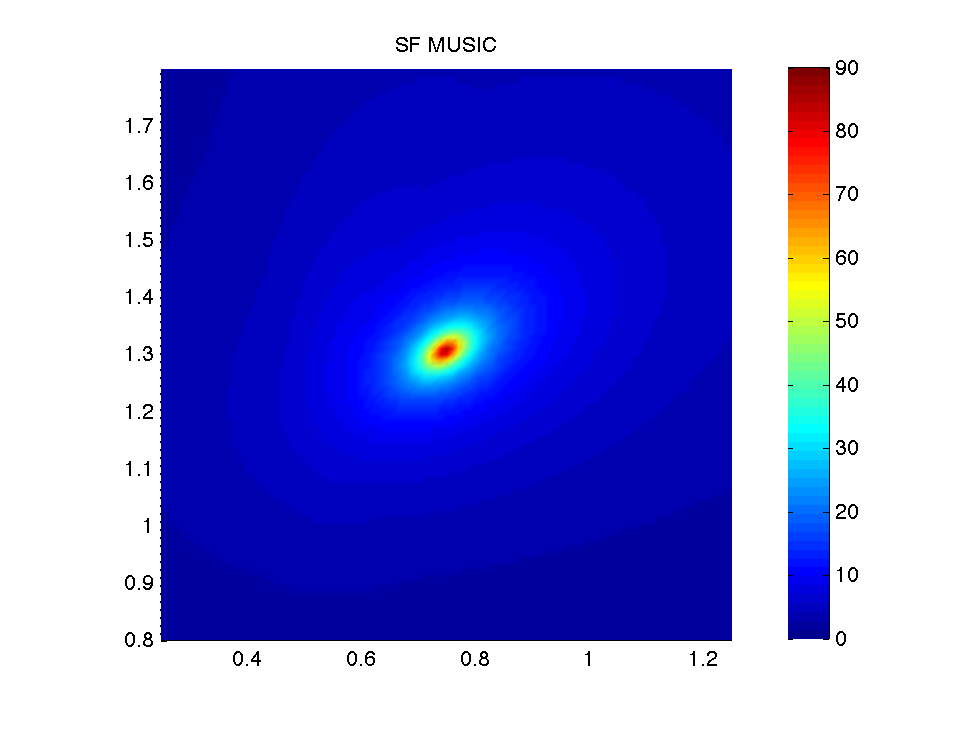
\includegraphics[width=7.cm]{model/disk.eps} \hspace{0.5cm}
\includegraphics[width=7.cm]{model/disk_geometry.eps}\\
& (a)\\ \tabularnewline  &
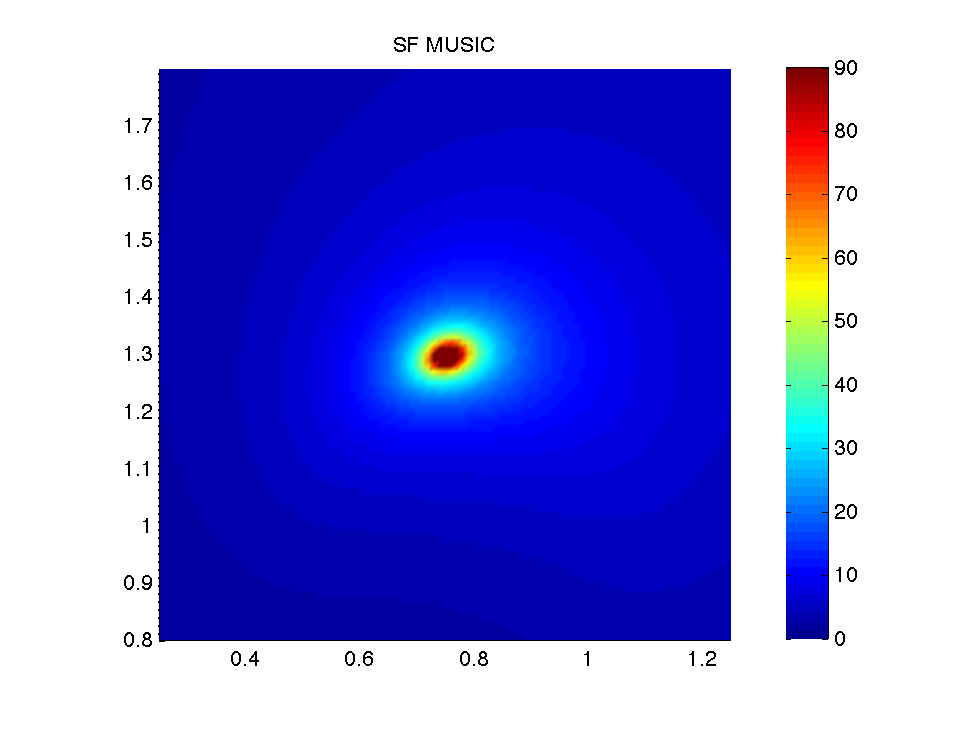
\includegraphics[width=7.cm]{model/ellipse.eps}
\hspace{0.5cm} 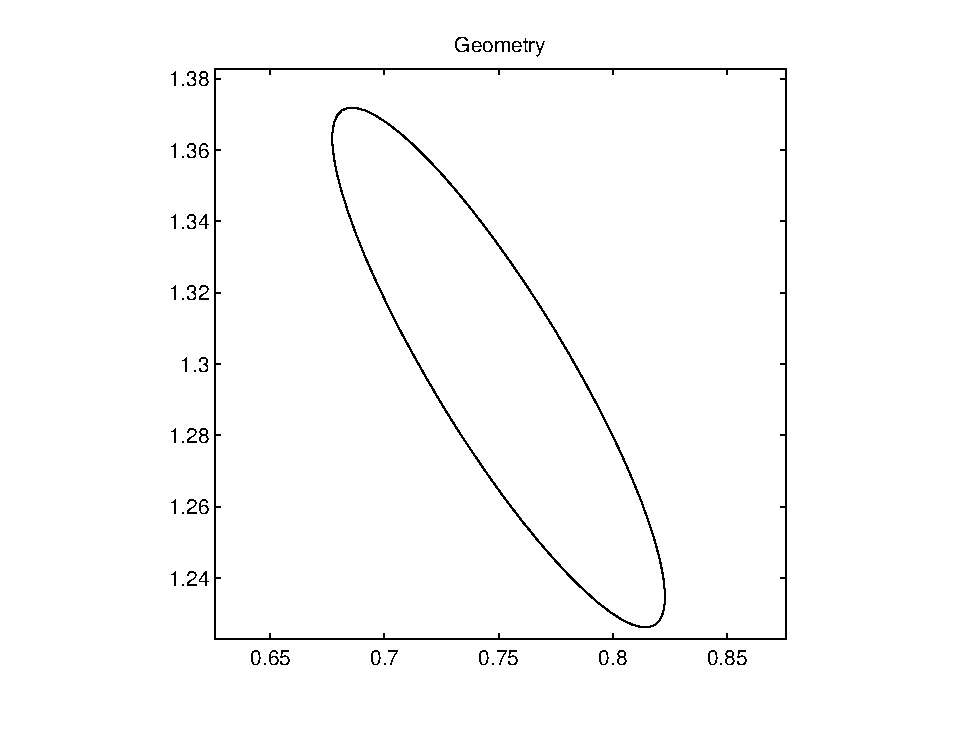
\includegraphics[width=7cm]{model/ellipse_geometry.eps} \\
& (b)\\ \tabularnewline  &
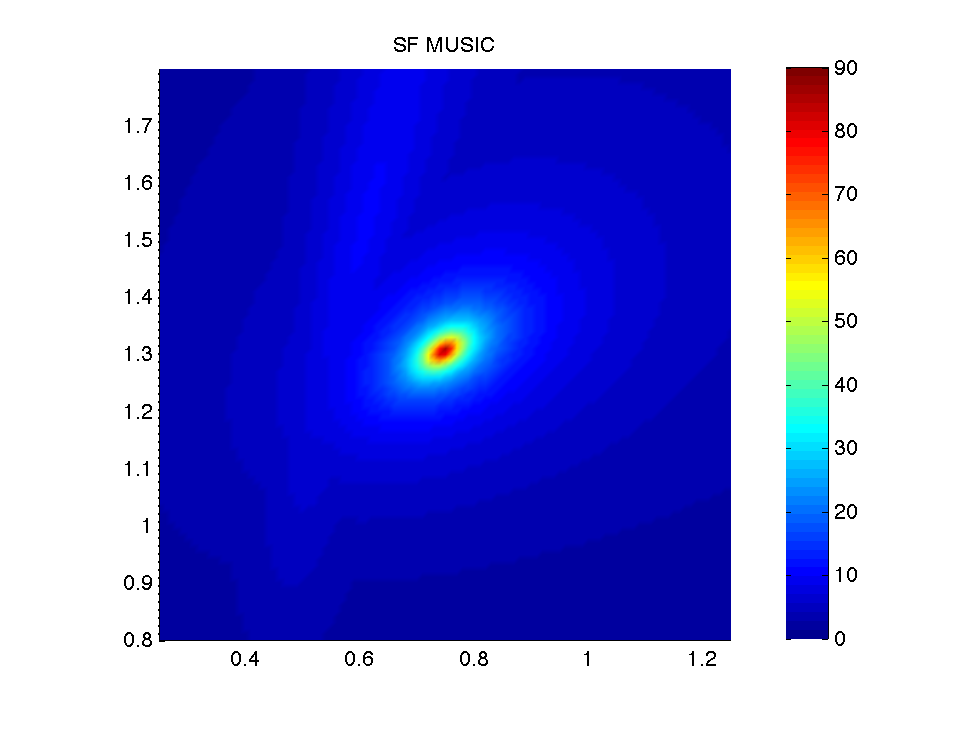
\includegraphics[width=7cm]{model/star.eps}
 \hspace{0.5cm} 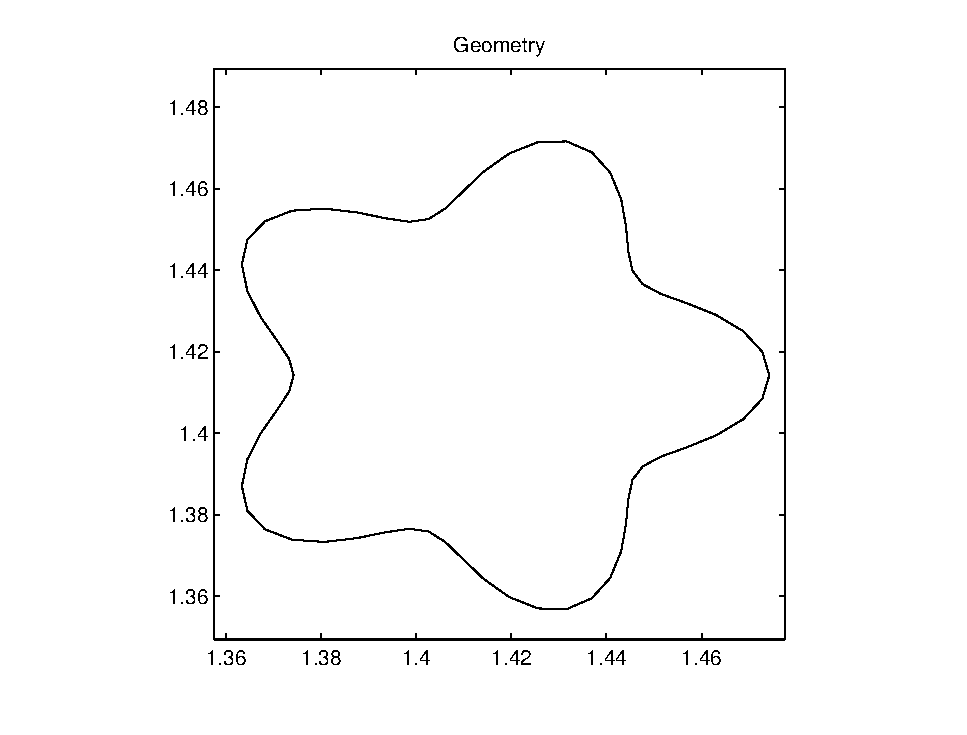
\includegraphics[width=7cm]{model/star_geometry.eps}\\
 & (c) \\
%\tabularnewline
%(a) & (b) & (c)\tabularnewline
\end{tabular}
\caption{\label{fig:SF-MUSIC}Detection (left) of the target with
the SF-MUSIC algorithm, for different target shapes (right). Here,
the number of used frequencies is $10$, equidistributed from
$\omega_0$ to $10 \omega_0$, and there are $64$ equidistant
sensors on the fish.}
\end{figure}

For multiple targets, we only have developped the algorithm for disks, and we
suppose that we know in advance their number, see Figure~\ref{fig:2disks-SF-MUSIC}.
We can see in Figure~\ref{fig:2disks_SF_MUSIC_Close} that if the disks are too close, we cannot distinguish
them.

The generalization
for other shapes would involve first to count the number of objects, by counting
the number of significant singular values~\cite{ammari2004reconstruction}. Then,
we would have to check for each singular value -~or each pair of singular values for
non-isotropic objects~- if it corresponds to an abject or not. An example of such
algorithm can be found in~\cite{mosher1999source}, where it has been called
\emph{Recursively Applied and Projected (RAP) MUSIC}.

\begin{figure}[!h]
\centering%
\subfigure[$t = (-0.5,0)$]{\label{fig:2disks_SF_MUSIC}\includegraphics[width=.45\textwidth]{model/2disks.eps}}
\subfigure[$t = (-0.25,0)$]{\label{fig:2disks_SF_MUSIC_Close}\includegraphics[width=.45\textwidth]{model/2disks_close.eps}}
\caption{Detection of two disks, the first one being the same as in~\ref{fig:SF-MUSIC}(a), with conductivity
$\sigma = 5$ and permittivity $\varepsilon = 2$. The second one has the same radius, and is translated by
the vector $t$ indicated below each figure. It has conductivity $\sigma = 3$ and permittivity
$\varepsilon = 1$. Their centers are indicated by a square
\label{fig:2disks-SF-MUSIC}}
\end{figure}

Let us notice that, in the absence of noise, the number of
used frequencies does not change  significantly the image. Indeed,
we can see in Figure \ref{fig:no-noise}(a) that we can recover the
location of the target  with only one frequency for a single disk. For several
disks, one needs the same number of frequencies as the number of disks, see
Figure~\ref{fig:2disks_1freq} and Figure~\ref{fig:2disks_2freq}.

\begin{figure}[!h]
\centering
\subfigure[]{\label{fig:no-noise}\includegraphics[width=7cm]{model/1freq-no_noise.eps}}\\
\subfigure[]{\label{fig:2disks_1freq}\includegraphics[width=7cm]{model/2disks_1freq.eps}}
\subfigure[]{\label{fig:2disks_2freq}\includegraphics[width=7cm]{model/2disks_2freq.eps}}
\caption{Target detection in the absence of
noise.
(a)The target is the
disk in Figure~\ref{fig:SF-MUSIC}(a), with only one frequency $\omega_0=1$.
(b) The two disks of Figure~\ref{fig:2disks_SF_MUSIC},
with only one frequency $\omega_0=1$.
(c) The two disks of Figure~\ref{fig:2disks_SF_MUSIC},
with two frequencies $\omega_0=1$ and $\omega_0=2$.
In all these experiments, the number of
sensors stay the same.}
\end{figure}

\subsubsection*{Stability estimates with respect to measurement noise}

Let us now consider the effect of measurement noise on the
performance of the location search algorithm. We add to the
entries of the SFR matrix $A$ defined in (\ref{eq:SFR-final})
independent Gaussian random variables of mean $0$ and standard
deviation
\[
\sqrt{\zeta}\max_{r,f}\left|\left(\left.\frac{\partial
u_{f}}{\partial\nu}\right|_{+}-\left.\frac{\partial
U}{\partial\nu}\right|_{+}\right)(x_{r})\right|.
\]
The parameter $\zeta$ is the relative strength of the noise, and
will be given in percentage.

In Figure~\ref{fig:2disks_SF_MUSIC_1noise}, one can see that even with $1\%$ of
noise level, we cannot discriminate two disks that are well separated. Hence,
we will focus in this subsection on the stability for only one object. 

\begin{figure}[!h]
\centering
\includegraphics[width=.45\textwidth]{model/2disks_1noise.eps}
\caption{Target detection for the two disks of Figure~\ref{fig:2disks_SF_MUSIC}
with $1\%$ noise.\label{fig:2disks_SF_MUSIC_1noise}}
\end{figure}

Figure~\ref{fig:noise-freq_qualitative} shows that increasing the
number of frequencies stabilizes the image. The image on the left
in Figure \ref{fig:noise-freq_qualitative} corresponds to the same
configuration as in Figure \ref{fig:no-noise}, but with $10\%$ of
noise.

\begin{figure}
\centering%
%\begin{tabular}{cc}
\includegraphics[width=7cm]{model/disk_1freq_10noise.eps} \hspace{0.2cm}
\includegraphics[width=7cm]{model/disk_100freq_10noise.eps}\tabularnewline
%(a) & (b)\tabularnewline
%\end{tabular}
\caption{ \label{fig:noise-freq_qualitative}Influence of the
number of used frequencies on the stability. Here, the same target
as in Figure \ref{fig:no-noise} is imaged with $10\%$ of noise and
only one frequency ~$\omega_0=1$~ (left), ~$100$~frequencies
equidistributed from $\omega_0$ to $100 \omega_0$ (right), with
$64$ sensors. The disks plot the exact position, and the squares
plot the location of the maximum of the imaging functional.}
\end{figure}

 Figure \ref{generalshape} shows the performance of the
imaging algorithms for a target of a noncircular shape.
\begin{figure}
\centering%
%\begin{tabular}{cc}
\includegraphics[width=7cm]{model/star_1freq_no_noise.eps} \hspace{0.2cm}
\includegraphics[width=7cm]{model/star_1freq_10noise.eps} \hspace{0.2cm}
%\includegraphics[width=5cm]{.eps}
\tabularnewline
%(a) & (b)\tabularnewline
%\end{tabular}
\caption{\label{generalshape} The same target as in Figure
\ref{fig:SF-MUSIC}(c) is imaged with  only one frequency
~$\omega_0=1$~ and without noise (left), with $10\%$ of noise
(right). The disks plot the exact position, and the squares plot
the location of the maximum of the imaging functional.
%~$100$~frequencies equidistributed from $\omega_0$ to $100
%\omega_0$ and $10\%$ of noise (right).
}
\end{figure}







More quantitatively, we have computed the empirical root mean
square location error (between the exact location of the target
and the maximum of the imaging functional), for $N_{r}=250$
realizations. The root mean square location error is defined by
$\sqrt{\EE(|{z}^{\textrm{est}} - z|^2 )}$ with $\EE$ standing for the
expectation (mean value) and $z^{\textrm{est}}$ (resp. $z$) being the
estimated location (resp. the exact one).

Here, the same target as in Figure \ref{fig:no-noise} is
considered. Results are shown in
Figure~\ref{fig:stats-freq-noise}.

\begin{figure}
\centering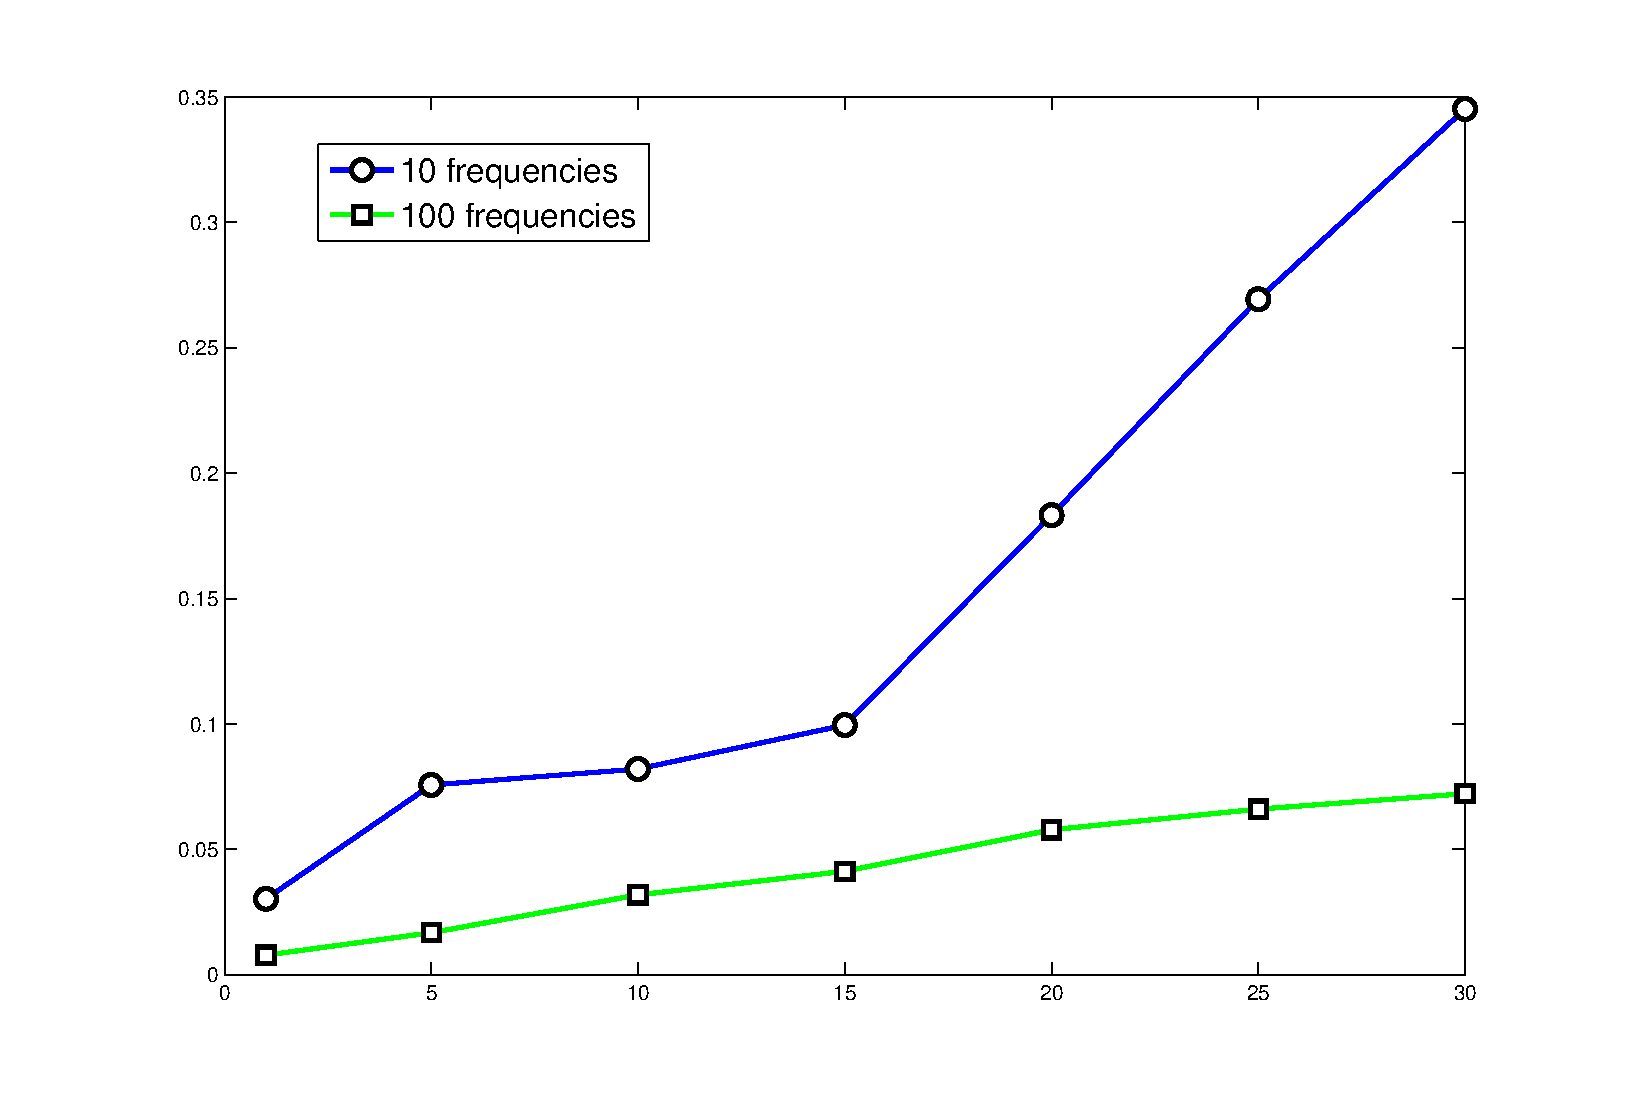
\includegraphics[height=7cm]{model/std_localization.eps}

\caption{\label{fig:stats-freq-noise}Influence of the number of
frequencies on the root mean square location error for $250$
realizations. Here, the horizontal axis is for the measurement
noise level in percentage and the vertical axis is for the root
mean square location error.}
\end{figure}

A natural question is whether taking different values for the
frequencies plays a role in the multi-frequency imaging procedure.
In order to answer this question, we construct an SFR matrix using
the same frequency for all the columns and compare the resulting
image with the one obtained using different frequencies (one for
each column). In Figure \ref{fig:noise-freq_100}, we use the data
obtained by $100$ trials (making measurements $100$ times using
the same frequency $\omega_0$) for $10\%$ of noise, $64$ sensors,
and a single frequency $\omega_0=1$. Here, the entries of each of
the $100$ columns are corrupted (independently) with $10\%$ of
noise. Figure \ref{fig:noise-freq_100} shows that the values of
the frequencies do not play a crucial role in the location
procedure. In fact, the location result is similar to the one in
Figure \ref{fig:noise-freq_qualitative}. However, from a practical
point of view, using simultaneously $N_f$ different frequencies
yields a faster robust location procedure than repeating $N_f$ times
the data acquisition procedure with the same frequency. In
subsection \ref{subsectcharcat}, we also identify the more
fundamental role of the values of the frequencies in the
characterization procedure.

\begin{figure}
\centering%
%\begin{tabular}{cc}
\includegraphics[width=7cm]{model/disk_100trials_10noise.eps} \hspace{0.2cm}
\includegraphics[width=7cm]{model/star_100trials_10noise.eps}
\caption{\label{fig:noise-freq_100} Influence of the values of
used frequencies on the stability. Imaging using the data obtained
by $100$ trials with $10\%$ of noise, $64$ sensors, and frequency
~$\omega_0=1$:  Left: the same target as in Figure
\ref{fig:SF-MUSIC}(a); Right: the same target as in Figure
\ref{fig:SF-MUSIC}(c). The disks plot the exact position, and the
squares plot the location of the maximum of the imaging
functional.}
\end{figure}



The number of sensors is also crucial in the stability of the
algorithm. Figure \ref{fig:stats-sensors-noise} compares the root
mean square location error with $100$ frequencies equidistributed
from $\omega_0$ to $100 \omega_0$ for $64$ and $8$ sensors for
different measurement noise levels.

\begin{figure}
\centering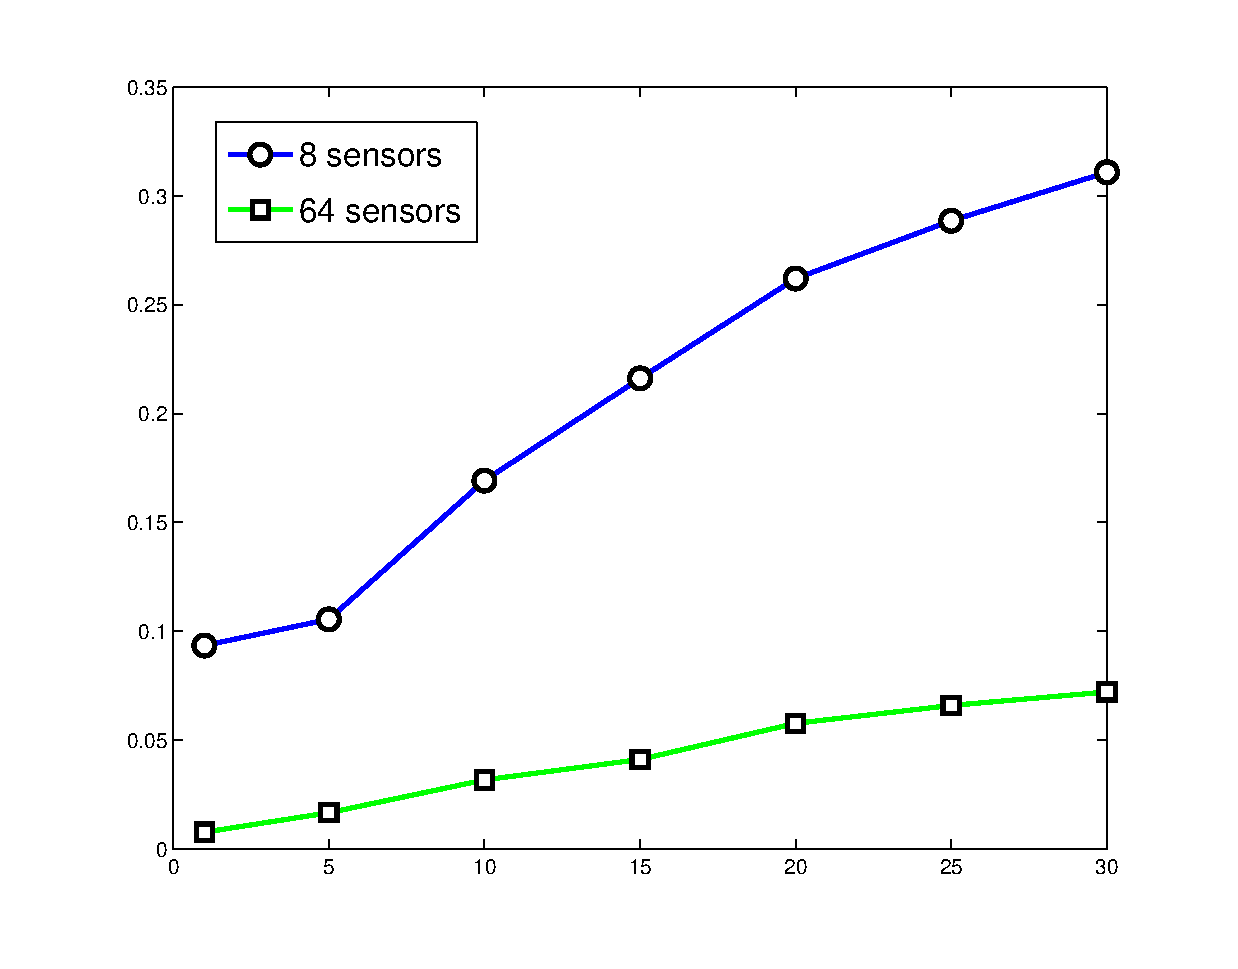
\includegraphics[height=8cm]{model/stats-sensors-noise.eps}\caption{\label{fig:stats-sensors-noise}Influence
of the number of sensors on the root mean square location error
for $250$ trials. Here, the horizontal axis is for the noise level
in percentage and the vertical axis is for the root mean square
location error.}
\end{figure}


The same type of statistics is possible for the detection as
function of the distance between the fish from the target. In
Figure~\ref{fig:distance-noise}, we have plotted the root mean
square location errors, with $15$ frequencies equidistributed from
$\omega_0$ to $15 \omega_0$  and $5\%$ of noise, for disks with
radius $0.05$ placed at $(t\cos(\pi/3),t\sin(\pi/3))$ for $t=1,
1.5, 2, 2.5,$ and $3$.

\begin{figure}


\centering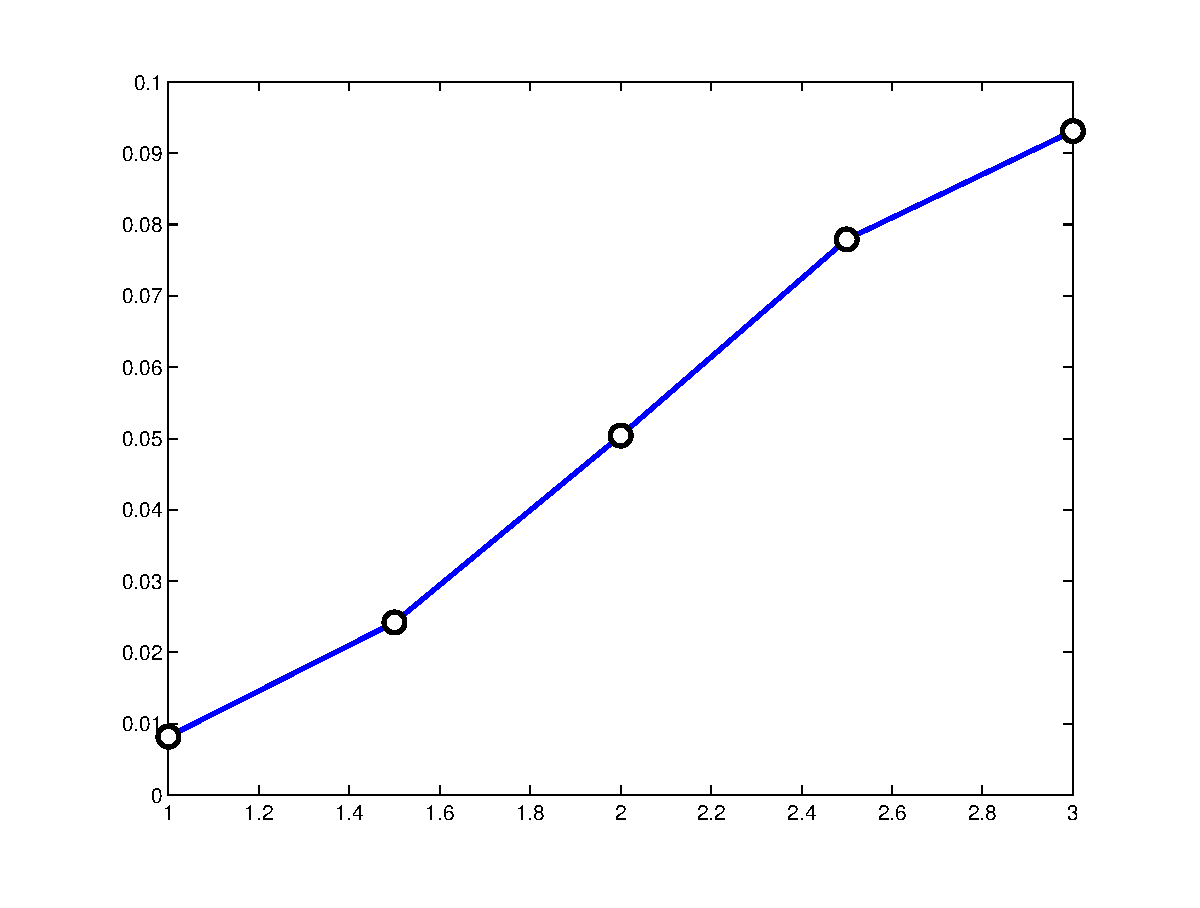
\includegraphics[width=10.5cm]{model/distance.eps}\caption{\label{fig:distance-noise}Influence
of the distance to the fish on the mean square location error for
$250$ trials. Here, the horizontal axis is for the distance to the
fish and the vertical axis is for the root mean square location
error.}


\end{figure}


%Finally, as we mentioned in section~\ref{sec:detection_algo}, the
%location of multiple targets is harder than the location of a
%single target. Indeed, in Figure~\ref{fig:svd-sfr} we have plotted
%the singular values of the response matrix $A$; the singular value
%decomposition (SVD) is used in our algorithm to compute the
%projection matrix onto the range of $A$. One can see that these
%values are extremely low, so that it is very hard to distinguish
%several targets. However, it should be possible to apply
%recursively this algorithm, as explained
%in~\cite{mosher1999source}.

%\begin{figure}


%\centering\includegraphics[width=8cm]{svd-sfr.eps}\caption{\label{fig:svd-sfr}Singular
%values of the post-treated response matrix (formula
%\ref{eq:SFR-final}), plotted in log-scale.}


%\end{figure}


\subsection{Target characterization} \label{subsectcharcat}

Once the target is located, one can use (\ref{eq:SFR-final}) to
estimate the electromagnetic parameters and the size of the
target. Assume that the target is a disk of radius $\delta$,
placed at $z$. From (\ref{eq:SFR-final}) it follows that
$\delta^2(k_f-1)/(k_f+1)$ can be estimated for $ 1\leq f \leq N_f$
from the measurement matrix $A$. Here, $k_f = k+i\varepsilon
\omega_0 f$ with $\omega_0$ being known. Let $\tau_r^{\mbox
{est}}$ be the estimated values of $\delta^2(k_f-1)/(k_f+1)$ from
$A$. To characterize the target and approximate its size, one
minimizes the following quadratic misfit functional:
\begin{equation} \label{minimiz1}
\sum_{1 \leq f\leq N_f} \bigg| \frac{\delta^2(k_f-1)}{k_f+1} -
\tau_r^{\mbox {est}} \bigg|^2,
\end{equation}
over $k, \varepsilon,$ and $\delta$.

Table \ref{table2} gives the result of the optimization algorithm
for a disk-shaped target with center center
$(1.5\cos(\pi/3),1.5\sin(\pi/3))$ and radius $\delta^{\textrm{true}}$. The electromagnetic parameters are $(\sigma^{{\textrm{true}}},
\varepsilon^{{\textrm{true}}})$. The initial guess is $\delta^{\textrm{init}} = 0.01, \sigma^{{\textrm{init}}} = 1, \varepsilon^{{\textrm{init}}}
=1.$ The data is collected for $100$ frequencies  equidistributed
from $\omega_0$ to $100 \omega_0$. The reconstructed results are
accurate.

\begin{table}[!h]
\centering
\begin{tabular}{|c|c|c||c|c|c|}
\hline $\delta^{{\textrm{true}}}$ & $\sigma^{{\textrm{true}}}$ &
$\varepsilon^{{\textrm{true}}}$ & $\delta^{{\textrm{est}}}$ & $\sigma^{\textrm{est}}$
 & $\varepsilon^{{\textrm{est}}}$\tabularnewline \hline 0.05 & 5
& 1 & 0.0506 & 4.9882 & 1.0004\tabularnewline \hline 0.05 & 4 & 1
& 0.0506 & 3.9993 & 0.9998\tabularnewline \hline 0.05 & 5 & 2 &
0.0506 & 4.9868 & 2.0017\tabularnewline \hline 0.06 & 5 & 1 &
0.0607 & 4.9878 & 1.0003\tabularnewline \hline 0.04 & 3 & 2 &
0.0404 & 2.9614 & 1.9806\tabularnewline \hline
\end{tabular}

\caption{Target characterization by minimizing the quadratic
misfit functional (\ref{minimiz1}) using data collected for $100$
frequencies equidistributed from $\omega_0$ to $100 \omega_0$.
Here, ${\textrm{true}}$: true values, ${\textrm{est}}$: estimated values.
The initial values are $\delta^{{\textrm{init}}} = 0.01, \sigma^{\textrm{init}} = 1,
 \varepsilon^{{\textrm{init}}} =1.$ \label{table2}}
\end{table}

When the target is an ellipse, the measurement matrix $A$ may not
be sufficient to characterize the electromagnetic parameters and
the size of the target. At least two different positions of the
fish (or equivalently two different locations of the target in the
fish frame of reference) are needed in order to generate
non-parallel dipole directions $\nabla U/|\nabla U|$ at the
location $z$ of the target and consequently lead to the extraction
of the polarization tensor $\mathbf{M}(\lambda_f, D)$ of the ellipse-shaped
target $D$. Consider two target locations $z_{1}$ and $z_{2}$ in
the fish frame of reference. Multi-frequency measurements lead to
two SFR matrices, $V_{rf}^{(1)}$ and $V_{rf}^{(2)}$ with $1\leq
r\leq N_r$ and $1\leq f\leq N_f$. Define the following linear
application from the set $\mathcal{M}$ of complex symmetric
$2\times 2$ matrices to $\mathbb{C}^{2N}$
\[
F: \mathbf{M} \mapsto\left(\begin{array}{c} \nabla
U(z_{1})^T  \mathbf{M}  \nabla_{z}\left(\left.\frac{\partial G}{\partial\nu_{x}}\right|_{+}\right)(x_{1},z_{1})\\
\vdots\\
\nabla U(z_{1})^T \mathbf{M}  \nabla_{z}\left(\left.\frac{\partial G}{\partial\nu_{x}}\right|_{+}\right)(x_{N_r},z_{1})\\
\nabla U(z_{2})^T \mathbf{M} \nabla_{z}\left(\left.\frac{\partial G}{\partial\nu_{x}}\right|_{+}\right)(x_{1},z_{2})\\
\vdots\\
\nabla U(z_{2})^T \mathbf{M} \nabla_{z}\left(\left.\frac{\partial
G}{\partial\nu_{x}}\right|_{+}\right)(x_{N_r},z_{2})
\end{array}\right)
.
\]
For a fixed $f$, we define the data
\[
b_{f}:=\left(\begin{array}{c}
\mathbf{V}_{1 f}^{(1)}\\
\vdots\\
\mathbf{V}_{Nr f}^{(1)}\\
\mathbf{V}_{1 f}^{(2)}\\
\vdots\\
\mathbf{V}_{Nr f}^{(2)}
\end{array}\right).
\]
By a least-squares method, we recover an estimation of the
polarization tensor $\mathbf{M}(\lambda_f,D)$:
\[
\mathbf{M}_{f}^{{\textrm{est}}}:=\arg\min_{\mathbf{M} \in \mathcal{M}}\left\Vert F(\mathbf{M})
-b_{f}\right\Vert .
\]
Again, once $\mathbf{M}(\lambda_f,D)$ is estimated, a minimization approach
yields correct parameter and size values. Since for any $f$, the
eigenvectors of the matrix $\mathbf{M}(\lambda_f,D)$ are the ellipse axes,
denoting $\tau_{f,1}^{\mbox {est}}$ and $\tau_{f,2}^{\mbox {est}}$
the estimated complex eigenvalues of $\mathbf{M}(\lambda_f,D)$, one minimizes the
following quadratic misfit functional
$$
\sum_{1\leq f\leq N_f} \bigg| \frac{a b (k_f-1) (a+b)}{a k_f+b} -
\tau_{f,1}^{\mbox {est}} \bigg|^2 + \bigg| \frac{a b (k_f-1)
(a+b)}{b k_f+a} - \tau_{f,2}^{\mbox {est}} \bigg|^2,
$$
over $a, b, k,$ and  $\varepsilon$, in order to reconstruct the
semi-axis lengths $a$ and $b$ and the material parameters $k$ and
$\varepsilon$ of the ellipse-shaped target $D$.


If $N_f$ is large enough, then semi-analytical formulas to estimate
the semi-axis lengths $a,b$ and the material parameters $k,
\varepsilon$ hold. Since
$$ \tau_{N_f,1}^{\mbox {est}} \approx \pi a(a+b),\quad  \tau_{N_f,2}^{\mbox {est}} \approx \pi
b(a+b),$$ one can estimate $a$ and $b$ as follows:
\begin{equation}
a^{\textrm{est}}  =\frac{\tau_{N_f,1}^{\mbox
{est}}}{\sqrt{\pi\left(\tau_{N_f,1}^{\mbox {est}} +\tau_{N_f,2}^{\mbox
{est}}\right)}},\quad  b^{\textrm{est}}  =\frac{\tau_{N_f,2}^{\mbox
{est}}}{\sqrt{\pi\left(\tau_{N_f,1}^{\mbox {est}}+\tau_{N_f,2}^{\mbox
{est}}\right)}}. \label{eq:estimation_parameters}
\end{equation}
Table~\ref{tab:characteriaztion_geometric_parameters} gives
 estimations of $a$ and $b$. The target is centered at $z_{1}=1.5(\cos(\pi/3),\sin(\pi/3))$
and the fish moves in the horizontal axis so that
$z_{2}=(1.5\cos(\pi/3)-1,1.5\sin(\pi/3))$. The material parameters
of the target are $k=2$ and $\varepsilon=1$.  The data is
collected for $10$ frequencies equidistributed from $\omega_0$ to
$10 \omega_0$. The reconstructed results are accurate.

\begin{table}[!h]
\centering%
\begin{tabular}{|c|c||c|c|}
\hline $a^{\textrm{true}}$ & $b^{\textrm{true}}$ & $a^{\textrm{est}}$ & $b^{\textrm{est}}$
\tabularnewline \hline \hline 0.04 & 0.04 & 0.0390 &
0.0405\tabularnewline \hline 0.05 & 0.05 & 0.0497 &
0.0516\tabularnewline \hline 0.05 & 0.06 & 0.0586 &
0.0608\tabularnewline \hline \hline 0.03 & 0.06 & 0.0313 &
0.0567\tabularnewline \hline 0.06 & 0.05 & 0.0406 &
0.0487\tabularnewline \hline 0.01 & 0.03 & 0.0108 &
0.0273\tabularnewline \hline
\end{tabular}
\caption{Estimations of the semi-axis lengths of ellipse-shaped
targets using
(\ref{eq:estimation_parameters}).\label{tab:characteriaztion_geometric_parameters}}
\end{table}

Moreover, once the geometric parameters $a$ and $b$ are estimated,
it is straightforward to recover $k$ and $\varepsilon$. Introduce
\[
\begin{alignedat}{1}\mu_{f}^{(1)} & :=\frac{\tau_{N_f,1}^{\mbox {est}}}{\pi ab(a+b)}=\frac{k_{f}-1}{a+k_{f}b}.\end{alignedat}
\]
From
\[
k_{f} = k+ i \varepsilon f \omega_0 =
\frac{1+a\mu_{f}^{(1)}}{1-b\mu_{f}^{(1)}},
\]
one can estimate $k$ and $\varepsilon$ as the real and imaginary
parts of $k_f$. However, as shown in
Figure~\ref{fig:param_phys_est}, one can see that the error on the
real part is growing with the frequency. Therefore, in order to
increase the robustness of the material parameter estimations, we
estimate $k$ using the lowest frequencies (for example the first
three) and $\varepsilon$ using all the frequencies:
\begin{equation}
k^{\textrm{est}} :=\frac{1}{3}\sum_{f=1}^{3}\Re\left(\frac{1+a^{\textrm{est}}
\mu_{f}^{(1)}}{1-b^{\textrm{est}}\mu_{f}^{(1)}}\right),\quad
\varepsilon^{\textrm{est}}
:=\frac{1}{N_f}\sum_{f=1}^{N_f}\frac{1}{\omega_{0}f}\Im\left(\frac{1+a^{\textrm{est}}
\mu_{f}^{(1)}}{1-b^{\textrm{est}}\mu_{f}^{(1)}}\right).
\label{eq:phys_param_est}
\end{equation}

\begin{figure}[!h]
\centering\includegraphics[width=8cm]{model/k_n_estimation}
\caption{\label{fig:param_phys_est}Conductivity, $k^{\textrm{est}}$, and
capacitance, $f \omega_0 \varepsilon^{\textrm{est}}$, of the
reconstructed conductivity (respectively represented by squares
and circles) for a disk-shaped target as functions of $f$ (\emph{
i.e.}, the frequency). Here, $\omega_0=1$ and the target is with
(true) material parameters $k=2$ and $\varepsilon=1$, radius
$0,05$, and placed at $z_{1}=1.5(\cos(\pi/3),\sin(\pi/3))$ and
then at $z_{2}=(1.5\cos(\pi/3)-1,1.5\sin(\pi/3))$. The solid lines
are the theoretical values.}
\end{figure}

Table~\ref{tab:param_phys_est} gives the material estimations
using formula (\ref{eq:phys_param_est}) for a disk and an ellipse.
Once again the results are accurate. Nevertheless, for high
contrasts between the real and imaginary parts of the 
admittivity the results of reconstruction are less satisfactory
(see also Figure~\ref{fig:param_phys_est}).

\begin{table}[!h]
\centering%
\begin{tabular}{|c||c|c||c|c|}
\cline{2-5} \multicolumn{1}{c|}{} & $k^{\textrm{true}}$ &
$\varepsilon^{\textrm{true}}$ & $k^{\textrm{est}}$ & $\varepsilon^{\textrm{est}}$
\tabularnewline \hline
 & 2 & 1 & 1.9167 & 1.0661\tabularnewline
\cline{2-5} disk & 3 & 2 & 2.8481 & 2.0516\tabularnewline
\cline{2-5}
 & 5 & 1 & 5.8884 & 1.4668\tabularnewline
\hline \hline
 & 2 & 1 & 1.7943 & 1.0473\tabularnewline
\cline{2-5} ellipse & 3 & 2 & 2.7208 & 2.0415\tabularnewline
\cline{2-5}
 & 5 & 1 & 6.0886 & 1.5828\tabularnewline
\hline
\end{tabular}

\caption{\label{tab:param_phys_est}Estimations of the material
parameters based on formula (\ref{eq:phys_param_est}). The disk
has radius $0,05$ and the ellipse has semi-axis lengths $0,025$
and $0,1$ and orientation angle $\pi/3$. Both targets are placed
at $z_{1}=1.5(\cos(\pi/3),\sin(\pi/3))$ and then at
$z_{2}=(1.5\cos(\pi/3)-1,1.5\sin(\pi/3))$, and are illuminated
with $10$ frequencies equidistributed from $\omega_0$ to $10
\omega_0$ (with $\omega_0=1$).}
\end{table}


\section{Concluding remarks}

In this chapter, we have proposed a non-iterative location
search algorithm based on multi-frequency measurements.  We have
presented some numerical results which are promising. We have seen
that increasing the number of frequencies (with not necessary
different values) improves the stability. In fact, using
multi-frequency measurements increases the signal-to-noise ratio.
On the other hand, using different frequencies yields a faster
robust location algorithm than repeating the data acquisition
procedure with the same frequency. We have also proposed a
procedure to reconstruct the electromagnetic parameters and the
size of disk- and ellipse-shaped targets. This has been possible
only because of multi-frequency measurements corresponding here to
different frequency values. The use of multi-frequency
measurements is fundamental in the characterization procedure. It
has been known that polarization tensor for real admittivities
(\ie for vanishing capacitance)
cannot separate the size from material properties of the target
\cite{ammari2007polarization}.

For arbitrary-shaped targets, many
important questions remain. In particular, it would be interesting
to know how much parameter and size information one can extract
from its polarization tensors for different
admittivities. A numerical answer will be provided in
chapter~\ref{chap:pnas}, but theoretical questions remain~\cite{kang2013IHP}.
It is also worth mentioning that limiting our
asymptotic expansions with respect to the target size to the
first-order term (the dipole approximation) does not give us the
shape of the target. Hence, in the next chapters we will
investigate how much information can be acquired in the near field
by approaching the fish next to the target and developing the
asymptotic expansions with high-order generalized polarization
tensors \cite{ammari2004reconstruction}.

% We will also investigate
% the stability of the proposed algorithm with respect to random
% fluctuations in the background permittivity and propose an
% original cross-correlation technique in order to correct for the
% effect of random heterogeneities on target location.

It is worth mentioning that in three dimensions the model problem and
the detection algorithm derived in this chapter is exactly the same
as in Proposition~\ref{proposition:SF-MUSIC}, see \cite{ammari2004reconstruction}.




